%!TEX root = ../StatisticalCorrelations.tex

\graphicspath{{Body/Figures/Correlations/}}

\section{Results}


-enter with how many jobs were submitted and how many succeeded, include a table of the number of samples, in the table include the Fiszher zed errors





\subsection{Correlation Results}




\begin{figure}[]
\centering
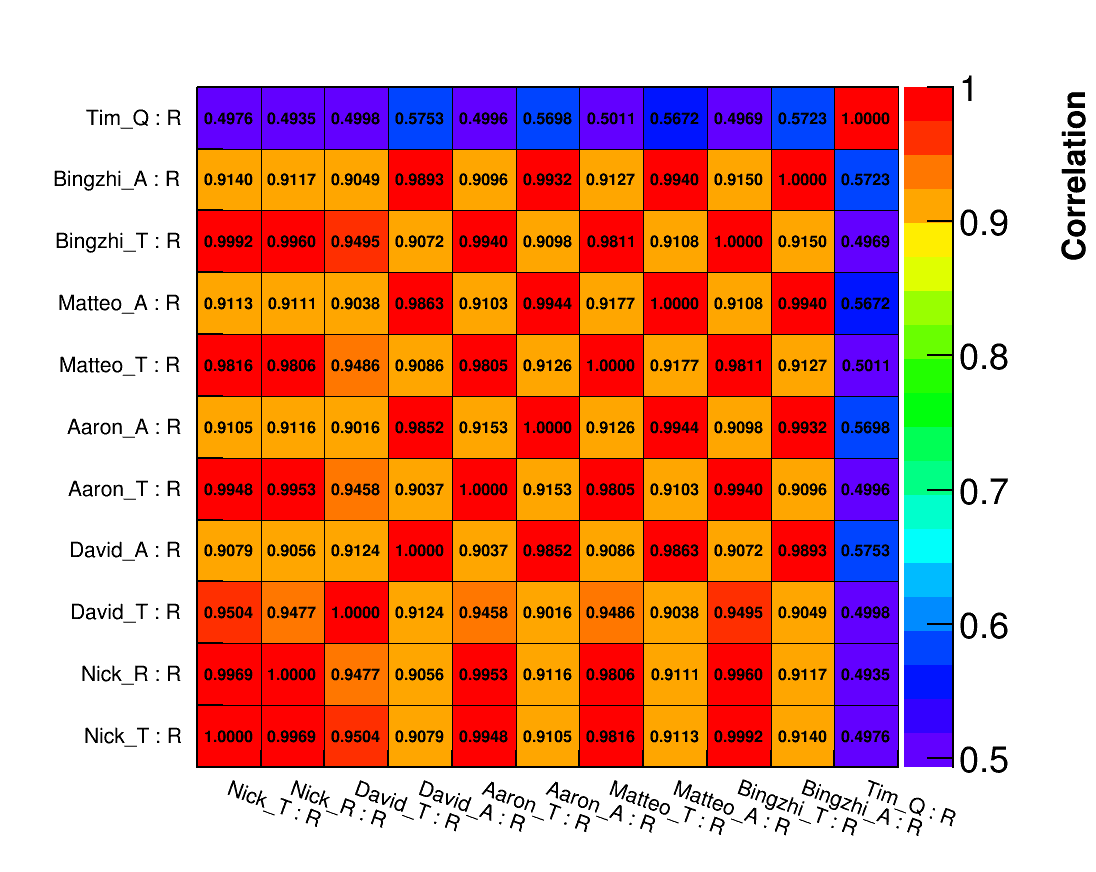
\includegraphics[width=\textwidth]{MethodType_CorrelationMatrixPlot_R_R_EG}
\caption{EG}
\label{fig:}
\end{figure}

\begin{figure}[]
\centering
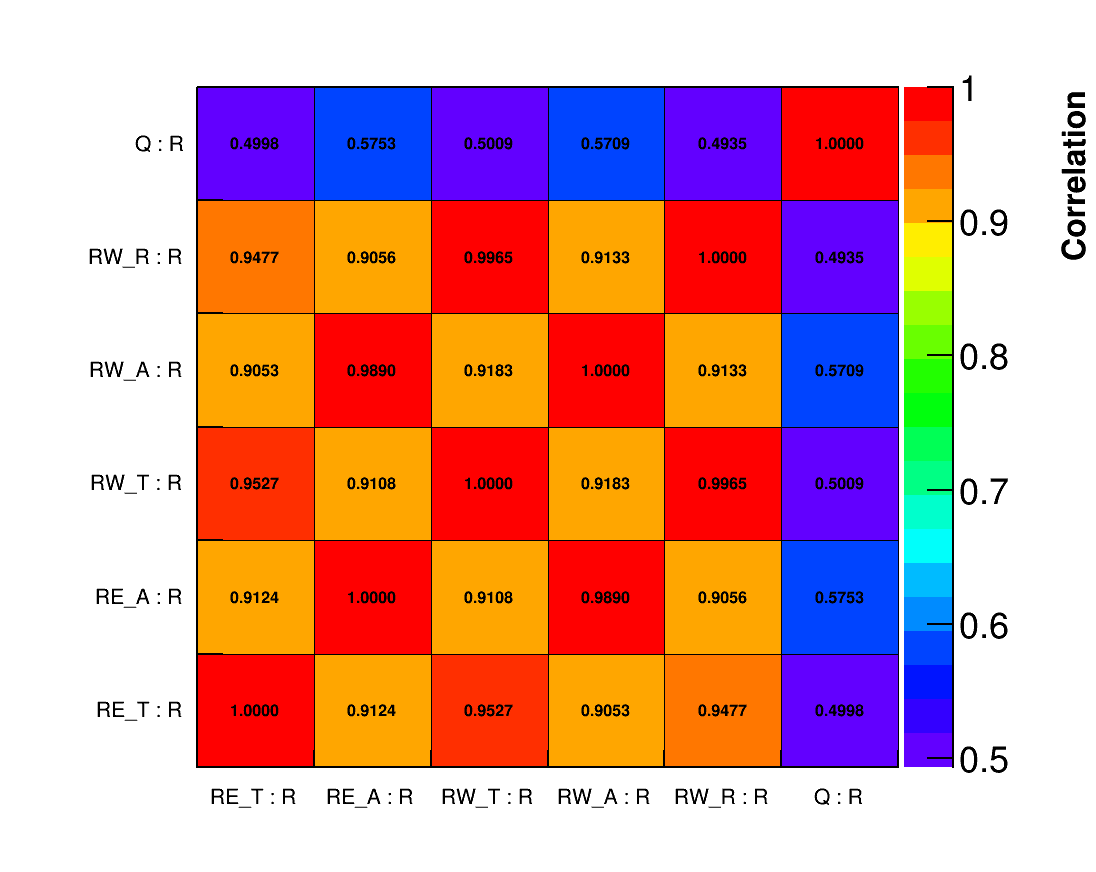
\includegraphics[width=\textwidth]{MethodType_Average_CorrelationMatrixPlot_R_R_EG}
\caption{EG}
\label{fig:}
\end{figure}


% 60h tables

\begin{table}
\footnotesize
\centering
\renewcommand{\arraystretch}{1.2}
\begin{tabular*}{1\linewidth}{@{\extracolsep{\fill}}lZZZZZZZZZZZ}
  \toprule
  	\multicolumn{12}{c}{60h Correlation Coefficients -- Analyzer Level -- Produced from \RE \texttt{TF2}} \\
  \midrule
  	       & \thead{BU T} & \thead{BU R} & \thead{CU T} & \thead{CU A} & \thead{UW T} & \thead{UW A} & \thead{EU T} & \thead{EU A} & \thead{SJTU T} & \thead{SJTU A} & \thead{UK Q} \\
  \midrule
	BU T   & 1.0000 & 0.9964 & 0.9460 & 0.9008 & 0.9936 & 0.8981 & 0.9783 & 0.9014 & 0.9992 & 0.9054 & 0.5071  \\
	BU R   & 0.9964 & 1.0000 & 0.9435 & 0.8989 & 0.9944 & 0.8995 & 0.9772 & 0.9015 & 0.9955 & 0.9032 & 0.5053  \\
	CU T   & 0.9460 & 0.9435 & 1.0000 & 0.9053 & 0.9408 & 0.8957 & 0.9418 & 0.8984 & 0.9451 & 0.9013 & 0.5072  \\
	CU A   & 0.9008 & 0.8989 & 0.9053 & 1.0000 & 0.8975 & 0.9840 & 0.9020 & 0.9858 & 0.9007 & 0.9896 & 0.5700  \\
	UW T   & 0.9936 & 0.9944 & 0.9408 & 0.8975 & 1.0000 & 0.9056 & 0.9771 & 0.9013 & 0.9927 & 0.9012 & 0.5095  \\
	UW A   & 0.8981 & 0.8995 & 0.8957 & 0.9840 & 0.9056 & 1.0000 & 0.9020 & 0.9935 & 0.8976 & 0.9914 & 0.5627  \\
	EU T   & 0.9783 & 0.9772 & 0.9418 & 0.9020 & 0.9771 & 0.9020 & 1.0000 & 0.9094 & 0.9774 & 0.9044 & 0.5144  \\
	EU A   & 0.9014 & 0.9015 & 0.8984 & 0.9858 & 0.9013 & 0.9935 & 0.9094 & 1.0000 & 0.9010 & 0.9934 & 0.5622  \\
	SJTU T & 0.9992 & 0.9955 & 0.9451 & 0.9007 & 0.9927 & 0.8976 & 0.9774 & 0.9010 & 1.0000 & 0.9065 & 0.5069  \\
	SJTU A & 0.9054 & 0.9032 & 0.9013 & 0.9896 & 0.9012 & 0.9914 & 0.9044 & 0.9934 & 0.9065 & 1.0000 & 0.5619  \\
	UK Q   & 0.5071 & 0.5053 & 0.5072 & 0.5700 & 0.5095 & 0.5627 & 0.5144 & 0.5622 & 0.5069 & 0.5619 & 1.0000  \\
  \bottomrule
\end{tabular*}
\caption[]{Correlation coefficients between \R values for individual analyses as determined for the 60h dataset with the \texttt{TF2} defined with the \RE energy binned functions.}
\label{tab:Corrs_60h_analyzer_EtW}
\end{table}

\begin{table}
\footnotesize
\centering
\renewcommand{\arraystretch}{1.2}
\begin{tabular*}{\linewidth}{@{\extracolsep{\fill}}lZZZZZZZZZZZ}
  \toprule
  	\multicolumn{12}{c}{60h Correlation Coefficient Differences -- Analyzer Level -- \RE \texttt{TF2} minus \RW \texttt{TF2}} \\
  \midrule
  	       & \thead{BU T} & \thead{BU R} & \thead{CU T} & \thead{CU A} & \thead{UW T} & \thead{UW A} & \thead{EU T} & \thead{EU A} & \thead{SJTU T} & \thead{SJTU A} & \thead{UK Q} \\
  \midrule
	BU T   & -0.0000 & 0.0001 & 0.0030 & 0.0032 & 0.0002 & 0.0007 & 0.0000 & 0.0001 & 0.0000 & 0.0008 & -0.0416  \\
	BU R   & 0.0001 & -0.0000 & 0.0035 & 0.0040 & 0.0002 & 0.0016 & -0.0009 & 0.0013 & -0.0002 & 0.0019 & -0.0405  \\
	CU T   & 0.0030 & 0.0035 & -0.0000 & 0.0019 & 0.0026 & 0.0049 & 0.0038 & 0.0042 & 0.0031 & 0.0042 & -0.0352  \\
	CU A   & 0.0032 & 0.0040 & 0.0019 & 0.0000 & 0.0005 & -0.0001 & 0.0042 & 0.0006 & 0.0044 & 0.0009 & -0.0453  \\
	UW T   & 0.0002 & 0.0002 & 0.0026 & 0.0005 & 0.0000 & -0.0019 & -0.0000 & -0.0024 & -0.0001 & -0.0019 & -0.0457  \\
	UW A   & 0.0007 & 0.0016 & 0.0049 & -0.0001 & -0.0019 & 0.0000 & 0.0009 & 0.0004 & 0.0011 & -0.0004 & -0.0600  \\
	EU T   & 0.0000 & -0.0009 & 0.0038 & 0.0042 & -0.0000 & 0.0009 & 0.0000 & 0.0005 & -0.0001 & 0.0008 & -0.0524  \\
	EU A   & 0.0001 & 0.0013 & 0.0042 & 0.0006 & -0.0024 & 0.0004 & 0.0005 & 0.0000 & 0.0007 & 0.0001 & -0.0612  \\
	SJTU T & 0.0000 & -0.0002 & 0.0031 & 0.0044 & -0.0001 & 0.0011 & -0.0001 & 0.0007 & 0.0000 & 0.0013 & -0.0404  \\
	SJTU A & 0.0008 & 0.0019 & 0.0042 & 0.0009 & -0.0019 & -0.0004 & 0.0008 & 0.0001 & 0.0013 & -0.0000 & -0.0547  \\
	UK Q   & -0.0416 & -0.0405 & -0.0352 & -0.0453 & -0.0457 & -0.0600 & -0.0524 & -0.0612 & -0.0404 & -0.0547 & 0.0000  \\
  \bottomrule
\end{tabular*}
\caption[]{Differences in the calculated correlation coefficients with the \texttt{TF2} defined with the \RE energy binned functions minus the \texttt{TF2} defined with the \RW energy binned functions, for the 60h dataset at the analyzer level.}
\label{tab:Corrs_60h_analyzer_diff_WtE}
\end{table}

\begin{table}
\setlength\tabcolsep{15pt}
\small
\centering
\renewcommand{\arraystretch}{1.2}
\begin{tabular*}{\linewidth}{@{\extracolsep{\fill}}lZZZZZZ}
  \toprule
  	\multicolumn{7}{c}{60h Correlation Coefficients -- Recon. Level -- Produced from \RE \texttt{TF2}} \\
  \midrule
  	       & \thead{RE T} & \thead{RE A} & \thead{RW T} & \thead{RW A} & \thead{RW R} & \thead{Q} \\
  \midrule
	RE T   & 1.0000 & 0.9053 & 0.9483 & 0.9006 & 0.9435 & 0.5072  \\
	RE A   & 0.9053 & 1.0000 & 0.9049 & 0.9889 & 0.8989 & 0.5700  \\
	RW T   & 0.9483 & 0.9049 & 1.0000 & 0.9097 & 0.9960 & 0.5121  \\
	RW A   & 0.9006 & 0.9889 & 0.9097 & 1.0000 & 0.9036 & 0.5636  \\
	RW R   & 0.9435 & 0.8989 & 0.9960 & 0.9036 & 1.0000 & 0.5053  \\
	Q      & 0.5072 & 0.5700 & 0.5121 & 0.5636 & 0.5053 & 1.0000  \\
  \bottomrule
\end{tabular*}
\caption[]{Correlation coefficients between \R values for individual analyses as determined for the 60h dataset with the \texttt{TF2} defined with the \RE energy binned functions, after the \RW T-Method and A-Method \R values were averaged among the different analyzers.}
\label{tab:Corrs_60h_recon_EtW}
\end{table}

\begin{table}
\setlength\tabcolsep{24pt}
\small
\centering
\renewcommand{\arraystretch}{1.2}
\begin{tabular*}{\linewidth}{@{\extracolsep{\fill}}lZZZZZZ}
  \toprule
  	\multicolumn{7}{c}{60h Correlation Coefficient Differences -- Recon. Level -- \RE \texttt{TF2} minus \RW \texttt{TF2}} \\
  \midrule
  	       & \thead{RE T} & \thead{RE A} & \thead{RW T} & \thead{RW A} & \thead{RW R} & \thead{Q} \\
  \midrule
	RE T   & -0.0000 & 0.0019 & 0.0031 & 0.0044 & 0.0035 & -0.0352  \\
	RE A   & 0.0019 & 0.0000 & 0.0031 & 0.0005 & 0.0040 & -0.0453  \\
	RW T   & 0.0031 & 0.0031 & 0.0000 & 0.0001 & -0.0002 & -0.0453  \\
	RW A   & 0.0044 & 0.0005 & 0.0001 & 0.0000 & 0.0016 & -0.0588  \\
	RW R   & 0.0035 & 0.0040 & -0.0002 & 0.0016 & -0.0000 & -0.0405  \\
	Q      & -0.0352 & -0.0453 & -0.0453 & -0.0588 & -0.0405 & 0.0000  \\
  \bottomrule
\end{tabular*}
\caption[]{Differences in the calculated correlation coefficients with the \texttt{TF2} defined with the \RE energy binned functions minus the \texttt{TF2} defined with the \RW energy binned functions, for the 60h dataset at the reconstruction level.}
\label{tab:Corrs_60h_recon_diff_WtE}
\end{table}


% HK tables

\begin{table}
\footnotesize
\centering
\renewcommand{\arraystretch}{1.2}
\begin{tabular*}{1\linewidth}{@{\extracolsep{\fill}}lZZZZZZZZZZZ}
  \toprule
  	\multicolumn{12}{c}{HK Correlation Coefficients -- Analyzer Level -- Produced from \RE \texttt{TF2}} \\
  \midrule
  	       & \thead{BU T} & \thead{BU R} & \thead{CU T} & \thead{CU A} & \thead{UW T} & \thead{UW A} & \thead{EU T} & \thead{EU A} & \thead{SJTU T} & \thead{SJTU A} & \thead{UK Q} \\
  \midrule
	BU T   & 1.0000 & 0.9967 & 0.9492 & 0.8965 & 0.9942 & 0.8953 & 0.9810 & 0.8977 & 0.9992 & 0.9011 & 0.4925  \\
	BU R   & 0.9967 & 1.0000 & 0.9462 & 0.8954 & 0.9946 & 0.8973 & 0.9795 & 0.8983 & 0.9958 & 0.8996 & 0.4889  \\
	CU T   & 0.9492 & 0.9462 & 1.0000 & 0.8996 & 0.9436 & 0.8858 & 0.9421 & 0.8874 & 0.9483 & 0.8915 & 0.4799  \\
	CU A   & 0.8965 & 0.8954 & 0.8996 & 1.0000 & 0.8930 & 0.9849 & 0.8926 & 0.9850 & 0.8958 & 0.9896 & 0.5499  \\
	UW T   & 0.9942 & 0.9946 & 0.9436 & 0.8930 & 1.0000 & 0.9012 & 0.9796 & 0.8971 & 0.9932 & 0.8966 & 0.4996  \\
	UW A   & 0.8953 & 0.8973 & 0.8858 & 0.9849 & 0.9012 & 1.0000 & 0.8950 & 0.9940 & 0.8946 & 0.9923 & 0.5527  \\
	EU T   & 0.9810 & 0.9795 & 0.9421 & 0.8926 & 0.9796 & 0.8950 & 1.0000 & 0.9012 & 0.9803 & 0.8967 & 0.5085  \\
	EU A   & 0.8977 & 0.8983 & 0.8874 & 0.9850 & 0.8971 & 0.9940 & 0.9012 & 1.0000 & 0.8971 & 0.9935 & 0.5516  \\
	SJTU T & 0.9992 & 0.9958 & 0.9483 & 0.8958 & 0.9932 & 0.8946 & 0.9803 & 0.8971 & 1.0000 & 0.9020 & 0.4928  \\
	SJTU A & 0.9011 & 0.8996 & 0.8915 & 0.9896 & 0.8966 & 0.9923 & 0.8967 & 0.9935 & 0.9020 & 1.0000 & 0.5471  \\
	UK Q   & 0.4925 & 0.4889 & 0.4799 & 0.5499 & 0.4996 & 0.5527 & 0.5085 & 0.5516 & 0.4928 & 0.5471 & 1.0000  \\
  \bottomrule
\end{tabular*}
\caption[]{Correlation coefficients between \R values for individual analyses as determined for the HK dataset with the \texttt{TF2} defined with the \RE energy binned functions.}
\label{tab:Corrs_HK_analyzer_EtW}
\end{table}

\begin{table}
\footnotesize
\centering
\renewcommand{\arraystretch}{1.2}
\begin{tabular*}{\linewidth}{@{\extracolsep{\fill}}lZZZZZZZZZZZ}
  \toprule
  	\multicolumn{12}{c}{HK Correlation Coefficient Differences -- Analyzer Level -- \RE \texttt{TF2} minus \RW \texttt{TF2}} \\
  \midrule
  	       & \thead{BU T} & \thead{BU R} & \thead{CU T} & \thead{CU A} & \thead{UW T} & \thead{UW A} & \thead{EU T} & \thead{EU A} & \thead{SJTU T} & \thead{SJTU A} & \thead{UK Q} \\
  \midrule
	BU T   & 0.0000 & 0.0001 & 0.0045 & 0.0083 & 0.0006 & 0.0030 & 0.0022 & 0.0062 & 0.0001 & 0.0066 & -0.0114  \\
	BU R   & 0.0001 & -0.0000 & 0.0048 & 0.0094 & 0.0005 & 0.0036 & 0.0020 & 0.0070 & 0.0001 & 0.0073 & -0.0139  \\
	CU T   & 0.0045 & 0.0048 & 0.0000 & 0.0055 & 0.0057 & 0.0000 & 0.0025 & 0.0019 & 0.0050 & 0.0029 & -0.0227  \\
	CU A   & 0.0083 & 0.0094 & 0.0055 & 0.0000 & 0.0115 & 0.0019 & 0.0051 & 0.0008 & 0.0091 & 0.0007 & -0.0273  \\
	UW T   & 0.0006 & 0.0005 & 0.0057 & 0.0115 & -0.0000 & 0.0039 & 0.0041 & 0.0085 & 0.0005 & 0.0093 & -0.0039  \\
	UW A   & 0.0030 & 0.0036 & 0.0000 & 0.0019 & 0.0039 & 0.0000 & 0.0015 & 0.0011 & 0.0035 & 0.0010 & -0.0230  \\
	EU T   & 0.0022 & 0.0020 & 0.0025 & 0.0051 & 0.0041 & 0.0015 & -0.0000 & 0.0027 & 0.0024 & 0.0036 & 0.0036  \\
	EU A   & 0.0062 & 0.0070 & 0.0019 & 0.0008 & 0.0085 & 0.0011 & 0.0027 & 0.0000 & 0.0069 & 0.0000 & -0.0241  \\
	SJTU T & 0.0001 & 0.0001 & 0.0050 & 0.0091 & 0.0005 & 0.0035 & 0.0024 & 0.0069 & -0.0000 & 0.0073 & -0.0117  \\
	SJTU A & 0.0066 & 0.0073 & 0.0029 & 0.0007 & 0.0093 & 0.0010 & 0.0036 & 0.0000 & 0.0073 & 0.0000 & -0.0281  \\
	UK Q   & -0.0114 & -0.0139 & -0.0227 & -0.0273 & -0.0039 & -0.0230 & 0.0036 & -0.0241 & -0.0117 & -0.0281 & 0.0000  \\
  \bottomrule
\end{tabular*}
\caption[]{Differences in the calculated correlation coefficients with the \texttt{TF2} defined with the \RE energy binned functions minus the \texttt{TF2} defined with the \RW energy binned functions, for the HK dataset at the analyzer level.}
\label{tab:Corrs_HK_analyzer_diff_WtE}
\end{table}

\begin{table}
\setlength\tabcolsep{15pt}
\small
\centering
\renewcommand{\arraystretch}{1.2}
\begin{tabular*}{\linewidth}{@{\extracolsep{\fill}}lZZZZZZ}
  \toprule
  	\multicolumn{7}{c}{HK Correlation Coefficients -- Recon. Level -- Produced from \RE \texttt{TF2}} \\
  \midrule
  	       & \thead{RE T} & \thead{RE A} & \thead{RW T} & \thead{RW A} & \thead{RW R} & \thead{Q} \\
  \midrule
	RE T   & 1.0000 & 0.8996 & 0.9501 & 0.8903 & 0.9462 & 0.4799  \\
	RE A   & 0.8996 & 1.0000 & 0.8986 & 0.9887 & 0.8954 & 0.5499  \\
	RW T   & 0.9501 & 0.8986 & 1.0000 & 0.9041 & 0.9962 & 0.5006  \\
	RW A   & 0.8903 & 0.9887 & 0.9041 & 1.0000 & 0.9004 & 0.5517  \\
	RW R   & 0.9462 & 0.8954 & 0.9962 & 0.9004 & 1.0000 & 0.4889  \\
	Q      & 0.4799 & 0.5499 & 0.5006 & 0.5517 & 0.4889 & 1.0000  \\
  \bottomrule
\end{tabular*}
\caption[]{Correlation coefficients between \R values for individual analyses as determined for the HK dataset with the \texttt{TF2} defined with the \RE energy binned functions, after the \RW T-Method and A-Method \R values were averaged among the different analyzers.}
\label{tab:Corrs_HK_recon_EtW}
\end{table}

\begin{table}
\setlength\tabcolsep{24pt}
\small
\centering
\renewcommand{\arraystretch}{1.2}
\begin{tabular*}{\linewidth}{@{\extracolsep{\fill}}lZZZZZZ}
  \toprule
  	\multicolumn{7}{c}{HK Correlation Coefficient Differences -- Recon. Level -- \RE \texttt{TF2} minus \RW \texttt{TF2}} \\
  \midrule
  	       & \thead{RE T} & \thead{RE A} & \thead{RW T} & \thead{RW A} & \thead{RW R} & \thead{Q} \\
  \midrule
	RE T   & 0.0000 & 0.0055 & 0.0039 & 0.0014 & 0.0048 & -0.0227  \\
	RE A   & 0.0055 & 0.0000 & 0.0080 & 0.0009 & 0.0094 & -0.0273  \\
	RW T   & 0.0039 & 0.0080 & 0.0000 & 0.0045 & 0.0001 & -0.0062  \\
	RW A   & 0.0014 & 0.0009 & 0.0045 & 0.0000 & 0.0058 & -0.0253  \\
	RW R   & 0.0048 & 0.0094 & 0.0001 & 0.0058 & -0.0000 & -0.0139  \\
	Q      & -0.0227 & -0.0273 & -0.0062 & -0.0253 & -0.0139 & 0.0000  \\
  \bottomrule
\end{tabular*}
\caption[]{Differences in the calculated correlation coefficients with the \texttt{TF2} defined with the \RE energy binned functions minus the \texttt{TF2} defined with the \RW energy binned functions, for the HK dataset at the reconstruction level.}
\label{tab:Corrs_HK_recon_diff_WtE}
\end{table}


% 9d tables

\begin{table}
\footnotesize
\centering
\renewcommand{\arraystretch}{1.2}
\begin{tabular*}{1\linewidth}{@{\extracolsep{\fill}}lZZZZZZZZZZZ}
  \toprule
  	\multicolumn{12}{c}{9d Correlation Coefficients -- Analyzer Level -- Produced from \RE \texttt{TF2}} \\
  \midrule
  	       & \thead{BU T} & \thead{BU R} & \thead{CU T} & \thead{CU A} & \thead{UW T} & \thead{UW A} & \thead{EU T} & \thead{EU A} & \thead{SJTU T} & \thead{SJTU A} & \thead{UK Q} \\
  \midrule
	BU T   & 1.0000 & 0.9968 & 0.9459 & 0.8999 & 0.9943 & 0.8992 & 0.9805 & 0.9034 & 0.9993 & 0.9055 & 0.5041  \\
	BU R   & 0.9968 & 1.0000 & 0.9432 & 0.8982 & 0.9947 & 0.9005 & 0.9792 & 0.9029 & 0.9962 & 0.9034 & 0.4998  \\
	CU T   & 0.9459 & 0.9432 & 1.0000 & 0.9024 & 0.9417 & 0.8911 & 0.9430 & 0.8924 & 0.9457 & 0.8961 & 0.5070  \\
	CU A   & 0.8999 & 0.8982 & 0.9024 & 1.0000 & 0.8962 & 0.9838 & 0.8963 & 0.9844 & 0.8993 & 0.9892 & 0.5706  \\
	UW T   & 0.9943 & 0.9947 & 0.9417 & 0.8962 & 1.0000 & 0.9058 & 0.9781 & 0.9028 & 0.9936 & 0.9018 & 0.5127  \\
	UW A   & 0.8992 & 0.9005 & 0.8911 & 0.9838 & 0.9058 & 1.0000 & 0.8997 & 0.9934 & 0.8986 & 0.9924 & 0.5780  \\
	EU T   & 0.9805 & 0.9792 & 0.9430 & 0.8963 & 0.9781 & 0.8997 & 1.0000 & 0.9078 & 0.9797 & 0.9026 & 0.4951  \\
	EU A   & 0.9034 & 0.9029 & 0.8924 & 0.9844 & 0.9028 & 0.9934 & 0.9078 & 1.0000 & 0.9027 & 0.9938 & 0.5684  \\
	SJTU T & 0.9993 & 0.9962 & 0.9457 & 0.8993 & 0.9936 & 0.8986 & 0.9797 & 0.9027 & 1.0000 & 0.9062 & 0.5021  \\
	SJTU A & 0.9055 & 0.9034 & 0.8961 & 0.9892 & 0.9018 & 0.9924 & 0.9026 & 0.9938 & 0.9062 & 1.0000 & 0.5659  \\
	UK Q   & 0.5041 & 0.4998 & 0.5070 & 0.5706 & 0.5127 & 0.5780 & 0.4951 & 0.5684 & 0.5021 & 0.5659 & 1.0000  \\
  \bottomrule
\end{tabular*}
\caption[]{Correlation coefficients between \R values for individual analyses as determined for the 9d dataset with the \texttt{TF2} defined with the \RE energy binned functions.}
\label{tab:Corrs_9d_analyzer_EtW}
\end{table}

\begin{table}
\footnotesize
\centering
\renewcommand{\arraystretch}{1.2}
\begin{tabular*}{\linewidth}{@{\extracolsep{\fill}}lZZZZZZZZZZZ}
  \toprule
  	\multicolumn{12}{c}{9d Correlation Coefficient Differences -- Analyzer Level -- \RE \texttt{TF2} minus \RW \texttt{TF2}} \\
  \midrule
  	       & \thead{BU T} & \thead{BU R} & \thead{CU T} & \thead{CU A} & \thead{UW T} & \thead{UW A} & \thead{EU T} & \thead{EU A} & \thead{SJTU T} & \thead{SJTU A} & \thead{UK Q} \\
  \midrule
	BU T   & 0.0000 & 0.0006 & 0.0029 & 0.0174 & 0.0009 & 0.0115 & 0.0037 & 0.0164 & 0.0000 & 0.0143 & 0.0209  \\
	BU R   & 0.0006 & -0.0000 & 0.0035 & 0.0195 & 0.0007 & 0.0122 & 0.0021 & 0.0168 & 0.0006 & 0.0154 & 0.0218  \\
	CU T   & 0.0029 & 0.0035 & 0.0000 & 0.0044 & 0.0051 & 0.0013 & 0.0021 & 0.0036 & 0.0037 & 0.0035 & 0.0141  \\
	CU A   & 0.0174 & 0.0195 & 0.0044 & 0.0000 & 0.0204 & 0.0009 & 0.0118 & 0.0009 & 0.0180 & 0.0012 & -0.0006  \\
	UW T   & 0.0009 & 0.0007 & 0.0051 & 0.0204 & 0.0000 & 0.0135 & 0.0022 & 0.0195 & 0.0010 & 0.0177 & 0.0256  \\
	UW A   & 0.0115 & 0.0122 & 0.0013 & 0.0009 & 0.0135 & 0.0000 & 0.0063 & 0.0004 & 0.0120 & 0.0003 & 0.0061  \\
	EU T   & 0.0037 & 0.0021 & 0.0021 & 0.0118 & 0.0022 & 0.0063 & -0.0000 & 0.0113 & 0.0037 & 0.0105 & -0.0082  \\
	EU A   & 0.0164 & 0.0168 & 0.0036 & 0.0009 & 0.0195 & 0.0004 & 0.0113 & 0.0000 & 0.0166 & -0.0005 & -0.0027  \\
	SJTU T & 0.0000 & 0.0006 & 0.0037 & 0.0180 & 0.0010 & 0.0120 & 0.0037 & 0.0166 & -0.0000 & 0.0147 & 0.0215  \\
	SJTU A & 0.0143 & 0.0154 & 0.0035 & 0.0012 & 0.0177 & 0.0003 & 0.0105 & -0.0005 & 0.0147 & -0.0000 & 0.0017  \\
	UK Q   & 0.0209 & 0.0218 & 0.0141 & -0.0006 & 0.0256 & 0.0061 & -0.0082 & -0.0027 & 0.0215 & 0.0017 & -0.0000  \\
  \bottomrule
\end{tabular*}
\caption[]{Differences in the calculated correlation coefficients with the \texttt{TF2} defined with the \RE energy binned functions minus the \texttt{TF2} defined with the \RW energy binned functions, for the 9d dataset at the analyzer level.}
\label{tab:Corrs_9d_analyzer_diff_WtE}
\end{table}

\begin{table}
\setlength\tabcolsep{15pt}
\small
\centering
\renewcommand{\arraystretch}{1.2}
\begin{tabular*}{\linewidth}{@{\extracolsep{\fill}}lZZZZZZ}
  \toprule
  	\multicolumn{7}{c}{9d Correlation Coefficients -- Recon. Level -- Produced from \RE \texttt{TF2}} \\
  \midrule
  	       & \thead{RE T} & \thead{RE A} & \thead{RW T} & \thead{RW A} & \thead{RW R} & \thead{Q} \\
  \midrule
	RE T   & 1.0000 & 0.9024 & 0.9485 & 0.8952 & 0.9432 & 0.5070  \\
	RE A   & 0.9024 & 1.0000 & 0.9021 & 0.9881 & 0.8982 & 0.5706  \\
	RW T   & 0.9485 & 0.9021 & 1.0000 & 0.9093 & 0.9964 & 0.5059  \\
	RW A   & 0.8952 & 0.9881 & 0.9093 & 1.0000 & 0.9043 & 0.5721  \\
	RW R   & 0.9432 & 0.8982 & 0.9964 & 0.9043 & 1.0000 & 0.4998  \\
	Q      & 0.5070 & 0.5706 & 0.5059 & 0.5721 & 0.4998 & 1.0000  \\
  \bottomrule
\end{tabular*}
\caption[]{Correlation coefficients between \R values for individual analyses as determined for the 9d dataset with the \texttt{TF2} defined with the \RE energy binned functions, after the \RW T-Method and A-Method \R values were averaged among the different analyzers.}
\label{tab:Corrs_9d_recon_EtW}
\end{table}

\begin{table}
\setlength\tabcolsep{24pt}
\small
\centering
\renewcommand{\arraystretch}{1.2}
\begin{tabular*}{\linewidth}{@{\extracolsep{\fill}}lZZZZZZ}
  \toprule
  	\multicolumn{7}{c}{9d Correlation Coefficient Differences -- Recon. Level -- \RE \texttt{TF2} minus \RW \texttt{TF2}} \\
  \midrule
  	       & \thead{RE T} & \thead{RE A} & \thead{RW T} & \thead{RW A} & \thead{RW R} & \thead{Q} \\
  \midrule
	RE T   & 0.0000 & 0.0044 & 0.0028 & 0.0028 & 0.0035 & 0.0141  \\
	RE A   & 0.0044 & 0.0000 & 0.0163 & 0.0010 & 0.0195 & -0.0006  \\
	RW T   & 0.0028 & 0.0163 & 0.0000 & 0.0131 & 0.0003 & 0.0147  \\
	RW A   & 0.0028 & 0.0010 & 0.0131 & 0.0000 & 0.0148 & 0.0017  \\
	RW R   & 0.0035 & 0.0195 & 0.0003 & 0.0148 & -0.0000 & 0.0218  \\
	Q      & 0.0141 & -0.0006 & 0.0147 & 0.0017 & 0.0218 & -0.0000  \\
  \bottomrule
\end{tabular*}
\caption[]{Differences in the calculated correlation coefficients with the \texttt{TF2} defined with the \RE energy binned functions minus the \texttt{TF2} defined with the \RW energy binned functions, for the 9d dataset at the reconstruction level.}
\label{tab:Corrs_9d_recon_diff_WtE}
\end{table}


% EG tables

\begin{table}
\footnotesize
\centering
\renewcommand{\arraystretch}{1.2}
\begin{tabular*}{1\linewidth}{@{\extracolsep{\fill}}lZZZZZZZZZZZ}
  \toprule
  	\multicolumn{12}{c}{EG Correlation Coefficients -- Analyzer Level -- Produced from \RE \texttt{TF2}} \\
  \midrule
  	       & \thead{BU T} & \thead{BU R} & \thead{CU T} & \thead{CU A} & \thead{UW T} & \thead{UW A} & \thead{EU T} & \thead{EU A} & \thead{SJTU T} & \thead{SJTU A} & \thead{UK Q} \\
  \midrule
	BU T   & 1.0000 & 0.9969 & 0.9504 & 0.9079 & 0.9948 & 0.9105 & 0.9816 & 0.9113 & 0.9992 & 0.9140 & 0.4976  \\
	BU R   & 0.9969 & 1.0000 & 0.9477 & 0.9056 & 0.9953 & 0.9116 & 0.9806 & 0.9111 & 0.9960 & 0.9117 & 0.4935  \\
	CU T   & 0.9504 & 0.9477 & 1.0000 & 0.9124 & 0.9458 & 0.9016 & 0.9486 & 0.9038 & 0.9495 & 0.9049 & 0.4998  \\
	CU A   & 0.9079 & 0.9056 & 0.9124 & 1.0000 & 0.9037 & 0.9852 & 0.9086 & 0.9863 & 0.9072 & 0.9893 & 0.5753  \\
	UW T   & 0.9948 & 0.9953 & 0.9458 & 0.9037 & 1.0000 & 0.9153 & 0.9805 & 0.9103 & 0.9940 & 0.9096 & 0.4996  \\
	UW A   & 0.9105 & 0.9116 & 0.9016 & 0.9852 & 0.9153 & 1.0000 & 0.9126 & 0.9944 & 0.9098 & 0.9932 & 0.5698  \\
	EU T   & 0.9816 & 0.9806 & 0.9486 & 0.9086 & 0.9805 & 0.9126 & 1.0000 & 0.9177 & 0.9811 & 0.9127 & 0.5011  \\
	EU A   & 0.9113 & 0.9111 & 0.9038 & 0.9863 & 0.9103 & 0.9944 & 0.9177 & 1.0000 & 0.9108 & 0.9940 & 0.5672  \\
	SJTU T & 0.9992 & 0.9960 & 0.9495 & 0.9072 & 0.9940 & 0.9098 & 0.9811 & 0.9108 & 1.0000 & 0.9150 & 0.4969  \\
	SJTU A & 0.9140 & 0.9117 & 0.9049 & 0.9893 & 0.9096 & 0.9932 & 0.9127 & 0.9940 & 0.9150 & 1.0000 & 0.5723  \\
	UK Q   & 0.4976 & 0.4935 & 0.4998 & 0.5753 & 0.4996 & 0.5698 & 0.5011 & 0.5672 & 0.4969 & 0.5723 & 1.0000  \\
  \bottomrule
\end{tabular*}
\caption[]{Correlation coefficients between \R values for individual analyses as determined for the EG dataset with the \texttt{TF2} defined with the \RE energy binned functions.}
\label{tab:Corrs_EG_analyzer_EtW}
\end{table}

\begin{table}
\footnotesize
\centering
\renewcommand{\arraystretch}{1.2}
\begin{tabular*}{\linewidth}{@{\extracolsep{\fill}}lZZZZZZZZZZZ}
  \toprule
  	\multicolumn{12}{c}{EG Correlation Coefficient Differences -- Analyzer Level -- \RE \texttt{TF2} minus \RW \texttt{TF2}} \\
  \midrule
  	       & \thead{BU T} & \thead{BU R} & \thead{CU T} & \thead{CU A} & \thead{UW T} & \thead{UW A} & \thead{EU T} & \thead{EU A} & \thead{SJTU T} & \thead{SJTU A} & \thead{UK Q} \\
  \midrule
	BU T   & 0.0000 & 0.0002 & 0.0040 & 0.0182 & 0.0008 & 0.0147 & 0.0007 & 0.0171 & 0.0001 & 0.0176 & -0.0207  \\
	BU R   & 0.0002 & -0.0000 & 0.0051 & 0.0203 & 0.0011 & 0.0173 & 0.0014 & 0.0191 & 0.0001 & 0.0198 & -0.0197  \\
	CU T   & 0.0040 & 0.0051 & 0.0000 & 0.0049 & 0.0037 & -0.0016 & 0.0064 & 0.0019 & 0.0032 & 0.0008 & -0.0179  \\
	CU A   & 0.0182 & 0.0203 & 0.0049 & 0.0000 & 0.0199 & 0.0009 & 0.0209 & 0.0003 & 0.0183 & 0.0012 & -0.0017  \\
	UW T   & 0.0008 & 0.0011 & 0.0037 & 0.0199 & 0.0000 & 0.0157 & 0.0019 & 0.0191 & 0.0010 & 0.0201 & -0.0203  \\
	UW A   & 0.0147 & 0.0173 & -0.0016 & 0.0009 & 0.0157 & 0.0000 & 0.0176 & 0.0008 & 0.0145 & 0.0008 & -0.0075  \\
	EU T   & 0.0007 & 0.0014 & 0.0064 & 0.0209 & 0.0019 & 0.0176 & -0.0000 & 0.0191 & 0.0008 & 0.0193 & -0.0164  \\
	EU A   & 0.0171 & 0.0191 & 0.0019 & 0.0003 & 0.0191 & 0.0008 & 0.0191 & -0.0000 & 0.0171 & 0.0004 & -0.0066  \\
	SJTU T & 0.0001 & 0.0001 & 0.0032 & 0.0183 & 0.0010 & 0.0145 & 0.0008 & 0.0171 & 0.0000 & 0.0173 & -0.0220  \\
	SJTU A & 0.0176 & 0.0198 & 0.0008 & 0.0012 & 0.0201 & 0.0008 & 0.0193 & 0.0004 & 0.0173 & -0.0000 & -0.0022  \\
	UK Q   & -0.0207 & -0.0197 & -0.0179 & -0.0017 & -0.0203 & -0.0075 & -0.0164 & -0.0066 & -0.0220 & -0.0022 & 0.0000  \\
  \bottomrule
\end{tabular*}
\caption[]{Differences in the calculated correlation coefficients with the \texttt{TF2} defined with the \RE energy binned functions minus the \texttt{TF2} defined with the \RW energy binned functions, for the EG dataset at the analyzer level.}
\label{tab:Corrs_EG_analyzer_diff_WtE}
\end{table}

\begin{table}
\setlength\tabcolsep{15pt}
\small
\centering
\renewcommand{\arraystretch}{1.2}
\begin{tabular*}{\linewidth}{@{\extracolsep{\fill}}lZZZZZZ}
  \toprule
  	\multicolumn{7}{c}{EG Correlation Coefficients -- Recon. Level -- Produced from \RE \texttt{TF2}} \\
  \midrule
  	       & \thead{RE T} & \thead{RE A} & \thead{RW T} & \thead{RW A} & \thead{RW R} & \thead{Q} \\
  \midrule
	RE T   & 1.0000 & 0.9124 & 0.9527 & 0.9053 & 0.9477 & 0.4998  \\
	RE A   & 0.9124 & 1.0000 & 0.9108 & 0.9890 & 0.9056 & 0.5753  \\
	RW T   & 0.9527 & 0.9108 & 1.0000 & 0.9183 & 0.9965 & 0.5009  \\
	RW A   & 0.9053 & 0.9890 & 0.9183 & 1.0000 & 0.9133 & 0.5709  \\
	RW R   & 0.9477 & 0.9056 & 0.9965 & 0.9133 & 1.0000 & 0.4935  \\
	Q      & 0.4998 & 0.5753 & 0.5009 & 0.5709 & 0.4935 & 1.0000  \\
  \bottomrule
\end{tabular*}
\caption[]{Correlation coefficients between \R values for individual analyses as determined for the EG dataset with the \texttt{TF2} defined with the \RE energy binned functions, after the \RW T-Method and A-Method \R values were averaged among the different analyzers.}
\label{tab:Corrs_EG_recon_EtW}
\end{table}

\begin{table}
\setlength\tabcolsep{24pt}
\small
\centering
\renewcommand{\arraystretch}{1.2}
\begin{tabular*}{\linewidth}{@{\extracolsep{\fill}}lZZZZZZ}
  \toprule
  	\multicolumn{7}{c}{EG Correlation Coefficient Differences -- Recon. Level -- \RE \texttt{TF2} minus \RW \texttt{TF2}} \\
  \midrule
  	       & \thead{RE T} & \thead{RE A} & \thead{RW T} & \thead{RW A} & \thead{RW R} & \thead{Q} \\
  \midrule
	RE T   & 0.0000 & 0.0049 & 0.0040 & 0.0002 & 0.0051 & -0.0179  \\
	RE A   & 0.0049 & 0.0000 & 0.0191 & 0.0006 & 0.0203 & -0.0017  \\
	RW T   & 0.0040 & 0.0191 & 0.0000 & 0.0170 & 0.0004 & -0.0201  \\
	RW A   & 0.0002 & 0.0006 & 0.0170 & -0.0000 & 0.0186 & -0.0056  \\
	RW R   & 0.0051 & 0.0203 & 0.0004 & 0.0186 & -0.0000 & -0.0197  \\
	Q      & -0.0179 & -0.0017 & -0.0201 & -0.0056 & -0.0197 & 0.0000  \\
  \bottomrule
\end{tabular*}
\caption[]{Differences in the calculated correlation coefficients with the \texttt{TF2} defined with the \RE energy binned functions minus the \texttt{TF2} defined with the \RW energy binned functions, for the EG dataset at the reconstruction level.}
\label{tab:Corrs_EG_recon_diff_WtE}
\end{table}


% 60h - HK differences

\begin{table}
\footnotesize
\centering
\renewcommand{\arraystretch}{1.2}
\begin{tabular*}{\linewidth}{@{\extracolsep{\fill}}lZZZZZZZZZZZ}
  \toprule
  	\multicolumn{12}{c}{Correlation Coefficient Differences -- 60h minus HK -- Analyzer Level -- Produced from \RE \texttt{TF2}} \\
  \midrule
  	       & \thead{BU T} & \thead{BU R} & \thead{CU T} & \thead{CU A} & \thead{UW T} & \thead{UW A} & \thead{EU T} & \thead{EU A} & \thead{SJTU T} & \thead{SJTU A} & \thead{UK Q} \\
  \midrule
	BU T   & 0.0000 & -0.0003 & -0.0032 & 0.0043 & -0.0006 & 0.0028 & -0.0027 & 0.0038 & -0.0000 & 0.0043 & 0.0146  \\
	BU R   & -0.0003 & -0.0000 & -0.0027 & 0.0035 & -0.0002 & 0.0023 & -0.0023 & 0.0031 & -0.0003 & 0.0036 & 0.0164  \\
	CU T   & -0.0032 & -0.0027 & 0.0000 & 0.0057 & -0.0028 & 0.0099 & -0.0002 & 0.0109 & -0.0032 & 0.0098 & 0.0273  \\
	CU A   & 0.0043 & 0.0035 & 0.0057 & 0.0000 & 0.0045 & -0.0009 & 0.0094 & 0.0007 & 0.0049 & 0.0001 & 0.0201  \\
	UW T   & -0.0006 & -0.0002 & -0.0028 & 0.0045 & 0.0000 & 0.0044 & -0.0025 & 0.0043 & -0.0005 & 0.0046 & 0.0099  \\
	UW A   & 0.0028 & 0.0023 & 0.0099 & -0.0009 & 0.0044 & 0.0000 & 0.0070 & -0.0005 & 0.0030 & -0.0009 & 0.0100  \\
	EU T   & -0.0027 & -0.0023 & -0.0002 & 0.0094 & -0.0025 & 0.0070 & 0.0000 & 0.0082 & -0.0028 & 0.0078 & 0.0060  \\
	EU A   & 0.0038 & 0.0031 & 0.0109 & 0.0007 & 0.0043 & -0.0005 & 0.0082 & -0.0000 & 0.0039 & -0.0001 & 0.0106  \\
	SJTU T & -0.0000 & -0.0003 & -0.0032 & 0.0049 & -0.0005 & 0.0030 & -0.0028 & 0.0039 & 0.0000 & 0.0044 & 0.0141  \\
	SJTU A & 0.0043 & 0.0036 & 0.0098 & 0.0001 & 0.0046 & -0.0009 & 0.0078 & -0.0001 & 0.0044 & -0.0000 & 0.0148  \\
	UK Q   & 0.0146 & 0.0164 & 0.0273 & 0.0201 & 0.0099 & 0.0100 & 0.0060 & 0.0106 & 0.0141 & 0.0148 & -0.0000  \\
  \bottomrule
\end{tabular*}
\caption[]{Differences in the calculated correlation coefficients with the \texttt{TF2} defined with the \RE energy binned functions, for the 60h dataset minus the HK dataset, at the analyzer level.}
\label{tab:Corrs_60h_analyzer_diff_HK}
\end{table}

\begin{table}
\setlength\tabcolsep{24pt}
\small
\centering
\renewcommand{\arraystretch}{1.2}
\begin{tabular*}{\linewidth}{@{\extracolsep{\fill}}lZZZZZZ}
  \toprule
  	\multicolumn{7}{c}{Correlation Coefficient Differences -- 60h minus HK -- Recon. Level -- Produced from \RE \texttt{TF2}} \\
  \midrule
  	       & \thead{RE T} & \thead{RE A} & \thead{RW T} & \thead{RW A} & \thead{RW R} & \thead{Q} \\
  \midrule
	RE T   & 0.0000 & 0.0057 & -0.0018 & 0.0104 & -0.0027 & 0.0273  \\
	RE A   & 0.0057 & 0.0000 & 0.0063 & 0.0001 & 0.0035 & 0.0201  \\
	RW T   & -0.0018 & 0.0063 & 0.0000 & 0.0056 & -0.0002 & 0.0115  \\
	RW A   & 0.0104 & 0.0001 & 0.0056 & 0.0000 & 0.0032 & 0.0119  \\
	RW R   & -0.0027 & 0.0035 & -0.0002 & 0.0032 & -0.0000 & 0.0164  \\
	Q      & 0.0273 & 0.0201 & 0.0115 & 0.0119 & 0.0164 & -0.0000  \\
  \bottomrule
\end{tabular*}
\caption[]{Differences in the calculated correlation coefficients with the \texttt{TF2} defined with the \RE energy binned functions, for the 60h dataset minus the HK dataset, at the reconstruction level.}
\label{tab:Corrs_60h_recon_diff_HK}
\end{table}


% 60h - 9d differences

\begin{table}
\footnotesize
\centering
\renewcommand{\arraystretch}{1.2}
\begin{tabular*}{\linewidth}{@{\extracolsep{\fill}}lZZZZZZZZZZZ}
  \toprule
  	\multicolumn{12}{c}{Correlation Coefficient Differences -- 60h minus 9d -- Analyzer Level -- Produced from \RE \texttt{TF2}} \\
  \midrule
  	       & \thead{BU T} & \thead{BU R} & \thead{CU T} & \thead{CU A} & \thead{UW T} & \thead{UW A} & \thead{EU T} & \thead{EU A} & \thead{SJTU T} & \thead{SJTU A} & \thead{UK Q} \\
  \midrule
	BU T   & -0.0000 & -0.0004 & 0.0001 & 0.0009 & -0.0007 & -0.0012 & -0.0022 & -0.0020 & -0.0001 & -0.0000 & 0.0030  \\
	BU R   & -0.0004 & -0.0000 & 0.0003 & 0.0007 & -0.0003 & -0.0010 & -0.0021 & -0.0015 & -0.0006 & -0.0002 & 0.0056  \\
	CU T   & 0.0001 & 0.0003 & -0.0000 & 0.0028 & -0.0009 & 0.0046 & -0.0012 & 0.0060 & -0.0006 & 0.0052 & 0.0002  \\
	CU A   & 0.0009 & 0.0007 & 0.0028 & 0.0000 & 0.0012 & 0.0002 & 0.0057 & 0.0014 & 0.0013 & 0.0004 & -0.0007  \\
	UW T   & -0.0007 & -0.0003 & -0.0009 & 0.0012 & 0.0000 & -0.0002 & -0.0010 & -0.0015 & -0.0009 & -0.0006 & -0.0032  \\
	UW A   & -0.0012 & -0.0010 & 0.0046 & 0.0002 & -0.0002 & 0.0000 & 0.0023 & 0.0001 & -0.0010 & -0.0010 & -0.0154  \\
	EU T   & -0.0022 & -0.0021 & -0.0012 & 0.0057 & -0.0010 & 0.0023 & 0.0000 & 0.0017 & -0.0023 & 0.0018 & 0.0193  \\
	EU A   & -0.0020 & -0.0015 & 0.0060 & 0.0014 & -0.0015 & 0.0001 & 0.0017 & -0.0000 & -0.0017 & -0.0004 & -0.0062  \\
	SJTU T & -0.0001 & -0.0006 & -0.0006 & 0.0013 & -0.0009 & -0.0010 & -0.0023 & -0.0017 & 0.0000 & 0.0003 & 0.0049  \\
	SJTU A & -0.0000 & -0.0002 & 0.0052 & 0.0004 & -0.0006 & -0.0010 & 0.0018 & -0.0004 & 0.0003 & 0.0000 & -0.0040  \\
	UK Q   & 0.0030 & 0.0056 & 0.0002 & -0.0007 & -0.0032 & -0.0154 & 0.0193 & -0.0062 & 0.0049 & -0.0040 & 0.0000  \\
  \bottomrule
\end{tabular*}
\caption[]{Differences in the calculated correlation coefficients with the \texttt{TF2} defined with the \RE energy binned functions, for the 60h dataset minus the 9d dataset, at the analyzer level.}
\label{tab:Corrs_60h_analyzer_diff_9d}
\end{table}

\begin{table}
\setlength\tabcolsep{24pt}
\small
\centering
\renewcommand{\arraystretch}{1.2}
\begin{tabular*}{\linewidth}{@{\extracolsep{\fill}}lZZZZZZ}
  \toprule
  	\multicolumn{7}{c}{Correlation Coefficient Differences -- 60h minus 9d -- Recon. Level -- Produced from \RE \texttt{TF2}} \\
  \midrule
  	       & \thead{RE T} & \thead{RE A} & \thead{RW T} & \thead{RW A} & \thead{RW R} & \thead{Q} \\
  \midrule
	RE T   & -0.0000 & 0.0028 & -0.0002 & 0.0054 & 0.0003 & 0.0002  \\
	RE A   & 0.0028 & 0.0000 & 0.0027 & 0.0008 & 0.0007 & -0.0007  \\
	RW T   & -0.0002 & 0.0027 & 0.0000 & 0.0004 & -0.0004 & 0.0063  \\
	RW A   & 0.0054 & 0.0008 & 0.0004 & 0.0000 & -0.0008 & -0.0085  \\
	RW R   & 0.0003 & 0.0007 & -0.0004 & -0.0008 & -0.0000 & 0.0056  \\
	Q      & 0.0002 & -0.0007 & 0.0063 & -0.0085 & 0.0056 & 0.0000  \\
  \bottomrule
\end{tabular*}
\caption[]{Differences in the calculated correlation coefficients with the \texttt{TF2} defined with the \RE energy binned functions, for the 60h dataset minus the 9d dataset, at the reconstruction level.}
\label{tab:Corrs_60h_recon_diff_9d}
\end{table}


% 60h - EG differences

\begin{table}
\footnotesize
\centering
\renewcommand{\arraystretch}{1.2}
\begin{tabular*}{\linewidth}{@{\extracolsep{\fill}}lZZZZZZZZZZZ}
  \toprule
  	\multicolumn{12}{c}{Correlation Coefficient Differences -- 60h minus EG -- Analyzer Level -- Produced from \RE \texttt{TF2}} \\
  \midrule
  	       & \thead{BU T} & \thead{BU R} & \thead{CU T} & \thead{CU A} & \thead{UW T} & \thead{UW A} & \thead{EU T} & \thead{EU A} & \thead{SJTU T} & \thead{SJTU A} & \thead{UK Q} \\
  \midrule
	BU T   & -0.0000 & -0.0005 & -0.0044 & -0.0071 & -0.0012 & -0.0124 & -0.0033 & -0.0099 & 0.0000 & -0.0086 & 0.0095  \\
	BU R   & -0.0005 & -0.0000 & -0.0041 & -0.0068 & -0.0009 & -0.0120 & -0.0034 & -0.0096 & -0.0005 & -0.0085 & 0.0118  \\
	CU T   & -0.0044 & -0.0041 & 0.0000 & -0.0071 & -0.0050 & -0.0059 & -0.0068 & -0.0054 & -0.0044 & -0.0036 & 0.0074  \\
	CU A   & -0.0071 & -0.0068 & -0.0071 & 0.0000 & -0.0063 & -0.0013 & -0.0066 & -0.0005 & -0.0066 & 0.0003 & -0.0053  \\
	UW T   & -0.0012 & -0.0009 & -0.0050 & -0.0063 & 0.0000 & -0.0097 & -0.0034 & -0.0089 & -0.0012 & -0.0084 & 0.0099  \\
	UW A   & -0.0124 & -0.0120 & -0.0059 & -0.0013 & -0.0097 & 0.0000 & -0.0106 & -0.0009 & -0.0122 & -0.0017 & -0.0072  \\
	EU T   & -0.0033 & -0.0034 & -0.0068 & -0.0066 & -0.0034 & -0.0106 & 0.0000 & -0.0082 & -0.0037 & -0.0083 & 0.0134  \\
	EU A   & -0.0099 & -0.0096 & -0.0054 & -0.0005 & -0.0089 & -0.0009 & -0.0082 & 0.0000 & -0.0098 & -0.0007 & -0.0050  \\
	SJTU T & 0.0000 & -0.0005 & -0.0044 & -0.0066 & -0.0012 & -0.0122 & -0.0037 & -0.0098 & 0.0000 & -0.0085 & 0.0100  \\
	SJTU A & -0.0086 & -0.0085 & -0.0036 & 0.0003 & -0.0084 & -0.0017 & -0.0083 & -0.0007 & -0.0085 & 0.0000 & -0.0104  \\
	UK Q   & 0.0095 & 0.0118 & 0.0074 & -0.0053 & 0.0099 & -0.0072 & 0.0134 & -0.0050 & 0.0100 & -0.0104 & 0.0000  \\
  \bottomrule
\end{tabular*}
\caption[]{Differences in the calculated correlation coefficients with the \texttt{TF2} defined with the \RE energy binned functions, for the 60h dataset minus the EG dataset, at the analyzer level.}
\label{tab:Corrs_60h_analyzer_diff_EG}
\end{table}

\begin{table}
\setlength\tabcolsep{24pt}
\small
\centering
\renewcommand{\arraystretch}{1.2}
\begin{tabular*}{\linewidth}{@{\extracolsep{\fill}}lZZZZZZ}
  \toprule
  	\multicolumn{7}{c}{Correlation Coefficient Differences -- 60h minus EG -- Recon. Level -- Produced from \RE \texttt{TF2}} \\
  \midrule
  	       & \thead{RE T} & \thead{RE A} & \thead{RW T} & \thead{RW A} & \thead{RW R} & \thead{Q} \\
  \midrule
	RE T   & 0.0000 & -0.0071 & -0.0044 & -0.0047 & -0.0041 & 0.0074  \\
	RE A   & -0.0071 & 0.0000 & -0.0060 & -0.0001 & -0.0068 & -0.0053  \\
	RW T   & -0.0044 & -0.0060 & 0.0000 & -0.0086 & -0.0005 & 0.0112  \\
	RW A   & -0.0047 & -0.0001 & -0.0086 & 0.0000 & -0.0097 & -0.0073  \\
	RW R   & -0.0041 & -0.0068 & -0.0005 & -0.0097 & -0.0000 & 0.0118  \\
	Q      & 0.0074 & -0.0053 & 0.0112 & -0.0073 & 0.0118 & 0.0000  \\
  \bottomrule
\end{tabular*}
\caption[]{Differences in the calculated correlation coefficients with the \texttt{TF2} defined with the \RE energy binned functions, for the 60h dataset minus the EG dataset, at the reconstruction level.}
\label{tab:Corrs_60h_recon_diff_EG}
\end{table}

